\documentclass[preprint,review,12pt]{elsarticle}
\usepackage{amsmath,amssymb,amsthm}
\usepackage{graphicx}
\usepackage{booktabs}
\usepackage[T1]{fontenc}
\usepackage{url}
\usepackage{lineno}
\linenumbers
\newtheorem{proposition}{Proposition}
\journal{Knowledge-Based Systems}
\biboptions{numbers,sort&compress}

\begin{document}
\begin{frontmatter}
\title{Detectability and complementarity of feature and spatial-order anomalies in embedding lattices: analytical bounds and a two-stage pre-registered evaluation}
\author[a]{Leon Sandler\corref{cor1}}
\cortext[cor1]{Corresponding author. E-mail: sandler.leon@gmail.com; ORCID 0009-0007-4584-808X.}
\address[a]{Independent Researcher, Northbrook, IL, USA}

\begin{abstract}
Anomaly scores on lattices of embeddings, such as image patch embeddings, usually measure how rare the vector of a site is and cannot see ordinary vectors in the wrong places. We study when feature scores and spatial-order scores are complementary and how to combine them without labels. Five elementary propositions make the limits explicit: position-free scores are blind to rearrangements; a fixed aggregation window keeps an anomalous site only if its local anomaly occupancy exceeds a computable threshold; a directional dispersion statistic ignores straight walls between ordered domains; a site-wise maximum of calibrated ranks keeps every detection of either score at the cost of at most their combined false positives; and rotation-invariant local statistics cannot see the interior of a rotated patch. On synthetic lattices with both kinds of anomaly, every single score had a worst-type average precision of 0.10 or less on an independent generator, where the site-wise maximum of a feature and a spatial score reached 0.53; on the development generator the maximum beat two locally adaptive rules, and choosing one score per cohort could not serve mixed lattices. The evaluation was pre-registered in two stages. The first frozen rule referenced rarity to the whole cohort and failed on its test generator (0.046, against 0.26 for a generic fused baseline), because the lattices did not share one normal distribution. A revised rule, frozen before a third generator was scored, beat every single score and three fused baselines there and tied a contextual LOF baseline. All data are synthetic.
\end{abstract}

\begin{keyword}
anomaly detection \sep spatial outliers \sep embedding lattices \sep score fusion \sep detectability \sep pre-registration
\end{keyword}
\end{frontmatter}

\section{Introduction}
Many knowledge-based and perception systems represent their input as a grid of vectors: the embeddings of the patches of an image, the feature vectors of a sensor array, or the orientation field of an ordered material. Unsupervised anomaly detection on such data usually asks how unusual the vector of a site is, for example by its distance to the nearest members of a memory of normal embeddings \citep{Roth2022,Defard2021} or by density- and isolation-based outlier scores \citep{Breunig2000,Liu2008}; surveys cover the many variants \citep{Chandola2009,Ruff2021,Pang2021,Aggarwal2017}. Such scores are blind by construction to an anomaly that consists only of ordinary vectors in the wrong places. Detectors for \emph{spatial} or \emph{contextual} outliers compare a site with its neighbors instead \citep{Shekhar2003,Song2007,Schubert2014}, and benchmarks of logical anomalies in images show that arrangement errors are a practically relevant class \citep{Bergmann2022}. The two families are usually developed separately, and how they should be combined, and when either can work at all, is rarely made explicit.

This paper studies that question on lattices of embeddings with a combination of elementary analysis and controlled computation. It addresses three research questions.
\begin{description}
\item[RQ1] Under what conditions does a score that depends only on a site's embedding fail to detect an anomaly that a spatial-order statistic can detect, and vice versa?
\item[RQ2] How do the geometry of an anomaly, the size of the neighborhood and the coherence of the background determine whether spatial aggregation preserves an anomaly and whether a spatial-order statistic can see it?
\item[RQ3] Can a label-free, site-by-site fusion of the two kinds of score detect feature and arrangement anomalies that occur \emph{in the same lattice} more reliably than choosing one score per cohort, and is a locally adaptive fusion worth its complexity?
\end{description}

The study builds on an earlier version of this work, which proposed a similarity-weighted rarity score (channel A), a directional order statistic (channel B) and a cohort-level choice between them by a tail index, and evaluated them on scenarios of which most had been used during development. That design was criticized, rightly, for the dependence between development and test data, for the lack of independent validation and because a cohort-level choice cannot serve lattices that contain both kinds of anomaly. The present version keeps the earlier results only as motivation and replaces the evaluation.

\textbf{Contributions.} (i) Five analytical statements (Section~\ref{sec:theory}): position-free scores are blind to rearrangements; a fixed aggregation window preserves an anomalous site only if its local anomaly occupancy exceeds a threshold computable from the scores; the directional order statistic is insensitive to straight walls between ordered domains; a site-wise maximum of calibrated scores retains every detection of either channel at the cost of at most their combined false positives; and rotation-invariant local statistics cannot see the interior of a rotated patch. (ii) A detectability map over feature strength, arrangement disruption and background coherence (Experiment A). (iii) A comparison of seven label-free fusion rules on lattices with both kinds of anomaly, including two locally adaptive rules (Experiment B). (iv) A two-stage pre-registered evaluation on generators that were frozen before they were scored (Experiment C): the first frozen rule failed, for a reason that we identify, and a revised rule was then confirmed on a third generator. (v) Robustness and runtime measurements (Experiment D). The results are reported whether or not they favor the methods proposed in the earlier version, and several do not. All data are synthetic; Section~\ref{sec:discussion} states what this does and does not establish.

\section{Related work}
\textbf{Feature-space anomaly scores.} Nearest-neighbor distances to a memory bank of normal patch embeddings are the basis of strong industrial inspection methods \citep{Roth2022}; Gaussian models of patch embeddings \citep{Defard2021}, LOF \citep{Breunig2000} and isolation forests \citep{Liu2008} are other marginal scores. All of them assign a score to a vector, not to its placement, which is the property formalized in Proposition~\ref{prop:perm}.

\textbf{Spatial, contextual and logical anomalies.} Spatial outlier detection compares an attribute with the aggregate of its spatial neighbors \citep{Shekhar2003}; conditional (contextual) anomaly detection models behavioral attributes given contextual ones \citep{Song2007}; Schubert et al.~\citep{Schubert2014} unify local outlier methods by their notion of locality. In vision, logical anomalies, such as missing, misplaced or wrongly combined parts, have their own benchmark \citep{Bergmann2022} and dedicated models \citep{Batzner2024}. The directional statistic studied here is a contextual score of a specific kind: it measures the dispersion of the unit vectors around a site \citep{Mardia2000,Banerjee2005} and takes the minimum over four sub-windows, as the Kuwahara filter does for intensity variance \citep{Kuwahara1976}, so that walls between ordered domains do not count as disorder.

\textbf{Score aggregation and fusion.} Smoothing per-site scores over a window is routine in anomaly localization; edge-preserving weights \citep{Tomasi1998} avoid averaging across boundaries. Combining detectors is the subject of outlier ensembles \citep{Aggarwal2015}, where maximum and average combination are standard, and comparing scores from different detectors requires their calibration to a common scale \citep{Kriegel2011}; here cohort ranks provide that scale without labels. The contribution of this paper is not a new ensemble rule but the analysis of when the two channels are complementary, when aggregation destroys a channel's signal, and what a site-wise maximum costs.


\section{Setting, scores and analytical results}
\label{sec:theory}

\subsection{Embedding lattices and the two kinds of anomaly}
A lattice of embeddings assigns a unit vector $u_i\in S^{d-1}$ to every site $i$ of an $n\times n$ grid, for example the normalized embedding of an image patch or the local orientation of an ordered medium. A cohort is a set of such lattices that are assumed to be mostly normal. We distinguish two kinds of anomaly. A \emph{feature anomaly} is a site whose embedding is rare in the cohort. An \emph{arrangement anomaly} is a site whose embedding is ordinary but placed where it does not fit its neighbors: in the extreme case the embeddings of a region are permuted among the sites of that region, or exchanged with those of a distant region, so that the multiset of embeddings of the lattice is unchanged.

\subsection{Scores}
All scores are label-free and are converted to cohort ranks (numbers in $(0,1]$, uniform over the cohort), which makes them comparable without labels \citep{Kriegel2011}.

\emph{Marginal scores} depend only on the embedding of a site. The \emph{cohort rarity} is the mean cosine distance of $u_i$ to its $k=5$ nearest neighbors in a reference pool of 3000 embeddings drawn from the \emph{other} lattices of the cohort; $r_i$ denotes its rank. The \emph{within-lattice rarity} uses the $k=20$ nearest neighbors among the other sites of the same lattice. LOF ($k=20$) \citep{Breunig2000} and an isolation forest (100 trees) \citep{Liu2008} are fitted on the embeddings of each lattice. \emph{Channel A}, proposed in the earlier version of this work, aggregates the cohort rarity with similarity weights,
\begin{equation}
c_{ij}=\exp\!\bigl(-(1-u_i^{\top}u_j)/\tau\bigr),\qquad A_i=\frac{\sum_{j\in W_i}c_{ij}\,r_j}{\sum_{j\in W_i}c_{ij}},
\label{eq:simw}
\end{equation}
over the $w\times w$ window $W_i$ ($w=3$ unless stated), with $\tau$ the median of $1-u_i^{\top}u_j$ over lattice-adjacent pairs of the cohort, an edge-preserving filter of the bilateral type \citep{Tomasi1998}; the fixed mean ($c_{ij}\equiv1$) is its reference.

\emph{Spatial scores} compare a site with its neighbors. The spatial outlier statistic of Shekhar et al.~\citep{Shekhar2003}, here $S_i=\|u_i-\bar u_{N_8(i)}\|$ with $\bar u_{N_8(i)}$ the mean of the eight neighbors; the mean cosine distance of a site to its eight neighbors; the isotropic disorder $D_i=1-\|\bar u_{N_4(i)}\|$ over the four lattice neighbors; and \emph{channel B}, the directional disorder. For the four $(h+1)\times(h+1)$ quadrant windows $Q_i^1,\dots,Q_i^4$ that have $i$ as a corner ($h=(w-1)/2$),
\begin{equation}
B_i=\min_{q}\;\Bigl(1-\Bigl\|\tfrac{1}{|Q_i^q|}\sum_{j\in Q_i^q}u_j\Bigr\|\Bigr).
\label{eq:dir}
\end{equation}
The bracket is one minus the mean resultant length, the classical dispersion of unit vectors \citep{Mardia2000}; the minimum over sub-windows that contain the site is the construction of the Kuwahara filter \citep{Kuwahara1976}. A joint baseline, contextual LOF, applies LOF to the concatenation $[u_i,\bar u_{N_8(i)}]$, in the spirit of contextual anomaly detection \citep{Song2007}.

\emph{Fusion.} With $a_i$ and $b_i$ the cohort ranks of a marginal and a spatial score, the site-wise rules are
\begin{equation}
S_i^{\max}=\max(a_i,b_i),\qquad S_i^{\mathrm{OR}}=1-(1-a_i)(1-b_i),
\label{eq:fusion}
\end{equation}
the second being the probability that at least one of two independent uniform variables falls below the observed values. Two locally adaptive rules and the cohort-level selection of one channel by a tail index (the fusion of the earlier version) are defined in Section~\ref{sec:design}.

\subsection{Analytical results}
The five statements below are elementary, and we present them as tools rather than as deep results: they make explicit, under stated assumptions, why one channel cannot replace the other, when spatial aggregation erases an anomaly, why the directional statistic ignores domain walls, what fusion can cost, and why local statistics cannot see the interior of a rotated patch. Table~\ref{tab:props} lists the assumptions, and Section~\ref{sec:results} checks each statement numerically.

\begin{proposition}[Blindness of marginal detectors to rearrangement]
\label{prop:perm}
Let a score be a function $s_i=g(u_i;\mathcal{R})$ of the embedding of site $i$ and of a reference set $\mathcal{R}$ that does not depend on the positions of the sites of the lattice under test. If the embeddings of a set of sites $M$ are permuted among the sites of $M$, the multiset $\{s_i\}$ of scores of the lattice is unchanged. If, in addition, $M$ is placed independently of the embedding field and the field is stationary, the scores of the sites of $M$ have the same distribution as those of the other sites, and the expected area under the ROC curve for separating $M$ from the rest is $1/2$.
\end{proposition}
\begin{proof}
A permutation $\pi$ of $M$ maps the multiset $\{u_i\}$ onto itself, so $\{g(u_{\pi(i)};\mathcal{R})\}=\{g(u_i;\mathcal{R})\}$. Under stationarity and independent placement, the embedding at a site of $M$ after the permutation is again a draw from the stationary marginal distribution, so a randomly chosen anomalous site and a randomly chosen normal site have exchangeable scores, and $P(s_{\mathrm{anom}}>s_{\mathrm{norm}})+\tfrac12P(s_{\mathrm{anom}}=s_{\mathrm{norm}})=\tfrac12$.
\end{proof}
The proposition concerns the collection of scores and their distribution; the score at an individual location changes after the permutation. It covers every per-site score that ignores the lattice positions, including the $k$-nearest-neighbor rarity, LOF \citep{Breunig2000} and isolation forests \citep{Liu2008} on the embeddings. Spatial aggregation of such a score (channel A) is not covered, but it inherits the blindness when the aggregated score is itself unchanged in distribution; Section~\ref{sec:results} measures it.

\begin{proposition}[Occupancy condition for survival under a fixed window]
\label{prop:surv}
Assume a two-level score: $r_i=r_a$ on anomalous sites and $r_i=r_n<r_a$ on normal sites. For any binary anomaly mask $M$ and window $W_i$, the fixed-window mean is $\bar r_i=r_n+p_i\,(r_a-r_n)$ with the occupancy $p_i=|M\cap W_i|/|W_i|$, and an anomalous site stays above a threshold $\theta$ (for example the cohort's top-3\% quantile of $\bar r$) if and only if
\begin{equation}
p_i\;\ge\;p^{*}=\frac{\theta-r_n}{r_a-r_n}.
\label{eq:pstar}
\end{equation}
The share of anomalous sites that survive is therefore the share of anomalous sites whose occupancy reaches $p^{*}$, a purely geometric property of the mask.
\end{proposition}
\begin{proof}
$\bar r_i=|W_i|^{-1}\bigl(|M\cap W_i|\,r_a+(|W_i|-|M\cap W_i|)\,r_n\bigr)$; solve $\bar r_i\ge\theta$ for $p_i$.
\end{proof}
For a $3\times3$ window, a single anomalous site has $p_i=1/9$, a site in the interior of a block has $p_i=1$, and a site on the border of a block has $p_i\le 6/9$; with $p^{*}$ near one, only block interiors survive. The two-level model is a good description only when the anomalous scores are close to saturation; with weak anomalies the scores of anomalous sites are spread, $\bar r_a$ falls below $\theta$, the model predicts that nothing survives, and the few strongest anomalous sites survive anyway (Section~\ref{sec:results}). The similarity weights of Eq.~\eqref{eq:simw} raise the effective occupancy of an anomalous site because its anomalous neighbors carry most of the weight, which is why channel A preserves small anomalies (Section~\ref{sec:results}).

\begin{proposition}[Directional disorder at a domain wall]
\label{prop:wall}
Let site $i$ belong to a domain $\Omega$ and let the wall of $\Omega$ near $i$ be straight at the scale of the window, i.e.\ $\Omega$ contains the closed half-plane $\{x:\nu^{\top}(x-x_i)\ge0\}$ intersected with the window, for some unit normal $\nu$. Then at least one quadrant window $Q_i^q$ lies entirely in $\Omega$, namely the one whose two axis directions $(\sigma_y,\sigma_x)$ satisfy $\sigma_y\nu_y\ge0$ and $\sigma_x\nu_x\ge0$. Consequently $B_i\le\max_{Q\subset\Omega}\bigl(1-\|\bar u_Q\|\bigr)$, the dispersion of one quadrant of the domain itself, and $B_i=0$ if the domain is perfectly ordered, whereas the isotropic disorder $D_i$ includes neighbors from both sides of the wall.
\end{proposition}
\begin{proof}
Every offset $\delta=(\sigma_y a,\sigma_x b)$ with $a,b\in\{0,\dots,h\}$ of the chosen quadrant satisfies $\nu^{\top}\delta=a\,|\nu_y|+b\,|\nu_x|\ge0$, so every site of that quadrant lies in the half-plane and hence in $\Omega$. The minimum in Eq.~\eqref{eq:dir} is at most the value of that quadrant.
\end{proof}
The condition fails at sites where the domain is narrower than the quadrant, for example at the tip of a one-site-wide protrusion or at a corner where three domains meet; there channel B can respond to a wall. Inside a region whose embeddings have been shuffled, every quadrant contains unrelated vectors and $B_i$ is the dispersion of a random sample of $(h+1)^2$ of them, so the statistic separates disorganized regions from walls between organized ones. A coherent region of unusual embeddings has $B_i\approx0$: channel B is blind to it, and that is channel A's task.

\begin{proposition}[Cost and benefit of max fusion]
\label{prop:fuse}
Let $a_i,b_i$ be the cohort ranks of the two channels and flag a site when its score exceeds $t$. For max fusion, the flagged set is the union of the sets flagged by the two channels at the same $t$. Hence, for every anomaly type, the true-positive rate of max fusion is at least the larger of the two channels' rates, and its false-positive rate is at most the sum of theirs.
\end{proposition}
\begin{proof}
$\max(a_i,b_i)>t$ if and only if $a_i>t$ or $b_i>t$; apply the union bound to the normal sites.
\end{proof}
Max fusion therefore never loses a detection made by either channel at a fixed rank threshold, and its price is at most the added false positives of the other channel, at most a doubling when the channels' false positives are disjoint. In average precision, which integrates over thresholds, this price shows up as a loss relative to the better channel for each anomaly type; Section~\ref{sec:results} measures it.

\begin{proposition}[Rotated patches and rotation-invariant local statistics]
\label{prop:rot}
Let a local statistic $t_i=T(u_i;\{u_j\}_{j\in N(i)})$ be invariant under the symmetries of the square neighborhood $N(i)$ (rotations by $90^\circ$ act on $N(i)$ by permuting its sites). If a square patch $P$ is rotated by $90^\circ$, then every site $i$ of $P$ whose neighborhood lies inside $P$ receives exactly the value that the statistic had, before the rotation, at the site of $P$ that was moved to $i$. The multiset of values over the interior of $P$ is therefore unchanged, and only the sites on the border of $P$, whose neighborhoods straddle the patch boundary, can change.
\end{proposition}
\begin{proof}
The rotation maps the interior site $i'$ with its neighborhood onto $i$ with its neighborhood, and the embedding at each neighbor of $i$ is the embedding at the corresponding neighbor of $i'$, with the neighbor positions permuted by the rotation. By invariance, $t_i$ after the rotation equals $t_{i'}$ before it.
\end{proof}
All spatial scores above are invariant in this sense (they use the mean or the dispersion of the neighbors), and so are the marginal scores. A rotated patch of an oriented texture is therefore detectable by them only along its border, whatever the threshold: a score that sees the interior must use orientation-dependent, i.e.\ non-invariant, information about the arrangement.

\begin{table}[t]
\caption{Assumptions and scope of the analytical statements, and where each is checked.}
\label{tab:props}
\centering\small
\resizebox{\linewidth}{!}{\begin{tabular}{p{2.6cm}p{6.2cm}p{4.0cm}}
\toprule
Statement & Assumptions & Numerical check\\
\midrule
Prop.~\ref{prop:perm} (blindness) & score depends only on the site's embedding and a position-free reference; for the AUC statement, stationary field, region placed independently & AUC of rarity and LOF on rearranged regions, both generators\\
Prop.~\ref{prop:surv} (occupancy) & two-level score, fixed window, threshold read from the smoothed scores & predicted vs measured survival for five mask shapes\\
Prop.~\ref{prop:wall} (walls) & wall straight at the scale of the quadrant; domains wider than the quadrant & share of domain-wall sites among the top 3\% of each disorder statistic\\
Prop.~\ref{prop:fuse} (fusion) & site-wise maximum of cohort ranks & true- and false-positive rates at the top 3\%, per anomaly type\\
Prop.~\ref{prop:rot} (rotations) & statistic invariant to the symmetries of the neighborhood; patch larger than the neighborhood & AUC on the interior and on the border of rotated patches\\
\bottomrule
\end{tabular}}
\end{table}



\section{Experimental design}
\label{sec:design}
\subsection{Generators}
Table~\ref{tab:gen} summarizes the three generators. Every lattice has $32\times32$ sites and $d=16$ unless stated, and contains feature anomalies (label 1) and arrangement anomalies (label 2); a cohort is ten lattices of one condition.

\textbf{G1 (development).} A Gaussian random field with correlation length 3 (default) occupies the first $d/2$ dimensions, with independent noise (standard deviation 0.2) in all $d$; the normal embeddings therefore lie near a common subspace. A feature anomaly is a $3\times3$ block, a single site or a random-walk blob shifted by $s$ along a random unit direction of the complementary dimensions. An arrangement anomaly takes a fraction $\delta$ of the sites of a $6\times6$ block and permutes their embeddings without fixed points. Prevalences are 1.5\% (feature) and 3.5\% (arrangement). The strength levels $s\in\{1,1.5,2,2.5,3\}$ were set by a pilot on development seeds so that the unsmoothed rarity spans average precision (AP) 0.07 to 0.86.

\textbf{G2 (stage-1 confirmation).} Sphere-native: 5--10 Voronoi domains per lattice, each with its own random mean direction, a linear drift of that direction across the domain, and its own von Mises--Fisher concentration (log-uniform between 40 and 400); the lattice therefore has domain walls and heterogeneous coherence. Feature anomalies are random-walk blobs of 1--12 sites drawn around a direction at angle $\phi$ from the local domain mean; arrangement anomalies exchange the embeddings of a fraction $\delta$ of the sites of two distant blobs of 16--32 sites and reshuffle them, so that the multiset of embeddings of the lattice is unchanged. Each lattice draws its own domain directions, so the lattices do \emph{not} share one normal distribution; this property was not recognized as decisive before the test (Section~\ref{sec:stage1}).

\textbf{G3 (stage-2 confirmation).} An oriented texture: a latent vector $[\cos\varphi,\sin\varphi,0.6\cos\psi,0.6\sin\psi]$, with a stripe phase $\varphi$ of wavelength 8 sites and slowly varying orientation and a slowly varying texture code $\psi\in[0,0.6]$, is mapped into $d$ dimensions by a random linear map \emph{shared by all lattices} (a fixed encoder), plus noise, and normalized. Feature anomalies are blobs whose texture code lies 1.2 outside the normal range; arrangement anomalies are either shuffled exchanges between two blobs, as in G2, or $6\times6$ patches rotated by $90^\circ$, in which every embedding and every local neighborhood stays ordinary.

\begin{table}[t]
\caption{The generators and their role.}
\label{tab:gen}
\centering\footnotesize
\resizebox{\linewidth}{!}{\begin{tabular}{p{1.1cm}p{3.6cm}p{3.6cm}p{3.6cm}p{2.3cm}}
\toprule
 & Background & Feature anomaly & Arrangement anomaly & Role\\
\midrule
G1 & Gaussian field in a $d/2$-dim.\ subspace; shared across lattices & shift out of the subspace (blocks, sites, blobs) & permutation inside $6\times6$ blocks & development\\
G2 & Voronoi domains, von Mises--Fisher, drift; own directions per lattice & blob drawn at angle $\phi$ from the local mean & exchange between two distant blobs & stage-1 test\\
G3 & oriented texture through a shared encoder & blob with an out-of-range texture code & exchange between blobs, or $90^\circ$ rotated patch & stage-2 test\\
\bottomrule
\end{tabular}}
\end{table}

\subsection{Fusion rules compared on the development generator}
Besides the maximum and the OR of Eq.~\eqref{eq:fusion}, five rules were compared: the cohort-level \emph{selection} of one channel by the 97th percentile of its robust $z$-score (median and MAD) \citep{Rousseeuw1993}, the fusion of the earlier version; \emph{zmax}, the site-wise maximum of the two robust $z$-scores; \emph{lcOR}, the OR rule after channel B has been standardized against the median and MAD of its own $15\times15$ neighborhood (a local calibration intended for heterogeneous backgrounds); \emph{relmax}, $\max(a_i,(1-g_i)b_i)$ with $g_i$ the cohort rank of the local median of $B$ (down-weighting channel B where the background itself is disordered); and $\max(r_i,b_i)$ with the unsmoothed rarity in place of channel A.

\subsection{Metrics}
For each lattice, the AP of a score is computed separately for feature anomalies against normal sites and for arrangement anomalies against normal sites (the other anomaly type excluded), and for all anomalies together \citep{Davis2006}. The per-type APs are averaged over the lattices of a condition, and the \emph{worst-type AP} is the smaller of the two averages; it is the primary endpoint, because a detector for mixed lattices must find both kinds. Uncertainty is a paired bootstrap over lattices (2000 resamples) of the difference between two detectors.

\subsection{Protocol}
\emph{Stage 1.} On G1 only: a pilot (strength levels), Experiment A (detectability map; 20 lattices per cell, $5\times5$ cells and a coherence axis), and Experiment B (four mixed conditions, 30 lattices each). The rule for choosing the fusion was declared in the code before Experiment B: the better of max$(A,B)$ and OR$(A,B)$ by the mean worst-type AP over the four conditions, replaced by an adaptive rule only if that rule was better and its paired 95\% interval excluded zero. A first run of Experiment B showed the unsmoothed rarity above channel A, so max(rarity, $B$) was added as a candidate and the generic pair max(isolation forest, Shekhar) as a comparator, and Experiment B was run again; both runs are archived. The selected rule, the G2 conditions, seeds, endpoint and comparators, and the SHA-256 of the study code were then written to a freeze file and committed to version control (2026-11-17 02:01:17 UTC, tag \texttt{kbs-freeze}) before any G2 lattice was scored; the confirmation script refuses to run if the code differs from the frozen hash. Experiment C ran the frozen rule on three G2 conditions with 30 lattices each.

\emph{Stage 2.} After the stage-1 result, a post-hoc exploration on fresh seeds of the four G1 and the three G2 conditions (20 lattices each) compared all 24 pairs of a marginal score (cohort rarity, within-lattice rarity, LOF, isolation forest), a spatial score (channel B, Shekhar statistic, neighbor distance) and a fusion (max, OR); the selection criterion, the highest mean worst-type AP over the seven conditions, was committed before the exploration was run. The selected rule was frozen a second time (tag \texttt{kbs-freeze-2}, 2026-11-17 02:07:07 UTC) together with generator G3, which had been written but never scored, and evaluated on two G3 conditions and on fresh seeds of one G2 and one G1 condition, 30 lattices each.

\emph{Experiment D} (descriptive, after both freezes) varies one factor at a time on G3 or G2 (dimension, lattice size, feature prevalence, window, background coherence, noise; 10 lattices per setting) and records the runtime per lattice on a desktop computer (8 cores).



\section{Results}
\label{sec:results}
\subsection{Checks of the analytical statements}
\emph{Blindness (Prop.~\ref{prop:perm}).} On lattices that contain only rearranged regions, the AUC of the cohort rarity for the rearranged sites was 0.52 (G1) and 0.52 (G2), and that of LOF 0.52 and 0.49 (30 lattices each): chance, as the proposition requires.

\emph{Occupancy (Prop.~\ref{prop:surv}).} Table~\ref{tab:p2} compares the predicted share of feature-anomaly sites that survive the fixed $3\times3$ mean at the cohort's top 3\% with the measured share, for strong anomalies ($s=3$, mean anomalous rank 0.97--0.98). The occupancy model reproduces the ordering of the shapes (single sites, then blobs, then blocks) but underestimates the measured survival, for example 0.13 predicted against 0.28 measured for $3\times3$ blocks, because the ranks of normal neighbors are spread rather than equal to their mean. Similarity weighting kept 0.50 of the single sites and 0.75--0.85 of the larger shapes, close to the unsmoothed score. With weaker anomalies ($s=1.5$) the anomalous ranks are spread, the model predicts no survival at all, and 4--21\% of the anomalous sites survived anyway; the model is a description of the strong-anomaly regime.

\begin{table}[t]
\caption{Survival of feature-anomaly sites at the cohort's top 3\% (G1, $s=3$, 20 lattices per shape): threshold occupancy $p^{*}$ of Eq.~\eqref{eq:pstar}, predicted share of anomalous sites with occupancy $\ge p^{*}$, and measured shares above the top-3\% threshold of each score.}
\label{tab:p2}
\centering\footnotesize
\resizebox{\linewidth}{!}{\begin{tabular}{lccccc}
\toprule
Shape & $p^{*}$ & Predicted (fixed mean) & Fixed mean & Unsmoothed & Similarity-weighted\\
\midrule
single sites & 0.75 & 0.00 & 0.03 & 0.81 & 0.50 \\
$3\times3$ blocks & 0.79 & 0.13 & 0.28 & 0.85 & 0.85 \\
$6\times6$ blocks & 0.84 & 0.46 & 0.55 & 0.81 & 0.82 \\
blobs of 6 & 0.77 & 0.00 & 0.15 & 0.83 & 0.76 \\
blobs of 12 & 0.80 & 0.08 & 0.22 & 0.78 & 0.75 \\
\bottomrule
\end{tabular}}
\end{table}

\emph{Walls (Prop.~\ref{prop:wall}).} On G2 lattices without anomalies, 27\% of the sites lie on a domain wall. Among the top 3\% of each statistic, the share of wall sites was 69\% for channel B, against 100\% for the isotropic disorder, 100\% for the neighbor distance and 99\% for the Shekhar statistic. The quadrant minimum removed about a third of the wall responses, as the proposition predicts for straight walls; the rest lie at corners, junctions of three domains and strongly drifting domains, where its condition fails.

\emph{Fusion cost (Prop.~\ref{prop:fuse}).} On G3 lattices with shuffled regions, at the top 3\% of the cohort, the true-positive rate of max(isolation forest, Shekhar) for feature anomalies was 1.00 (channels: 1.00 and 0.01) and for arrangement anomalies 0.44 (0.02 and 0.43); its false-positive rate was 0.018, against 0.012 and 0.006 for the channels, i.e.\ close to their sum.

\emph{Rotations (Prop.~\ref{prop:rot}).} On G3 lattices with rotated patches (30 lattices), the mean AUC of the Shekhar statistic was 0.39 on the interior of the patches and 0.87 on their border; for the neighbor distance 0.41 and 0.82, and for contextual LOF 0.40 and 0.91. No statistic did better than chance on the interior. Channel B did not see the border either (0.40 and 0.51): the seam of a rotated patch is a wall between two ordered regions, which the quadrant minimum ignores by construction (Prop.~\ref{prop:wall}).

\subsection{Experiment A: the detectability map}
Figure~\ref{fig:phase} shows the AP of each channel for its own anomaly type and the worst-type AP of max$(A,B)$ over feature strength and arrangement disruption on G1. Every single score has a worst-type AP of at most 0.10 in every cell, because it is blind to the other type, whereas the maximum reaches up to 0.53. The feature AP of channel A is set by $s$ and hardly depends on $\delta$, and the arrangement AP of channel B grows with $\delta$ and is independent of $s$: the two channels respond to separate axes. A more coherent background helps neither: as the correlation length grows from 1 to 6 sites, the arrangement AP of channel B falls from 0.78 to 0.53, because a shuffle among nearly identical vectors changes little, and the feature AP of channel A falls from 0.69 to 0.30.

\begin{figure*}[t]
\centering
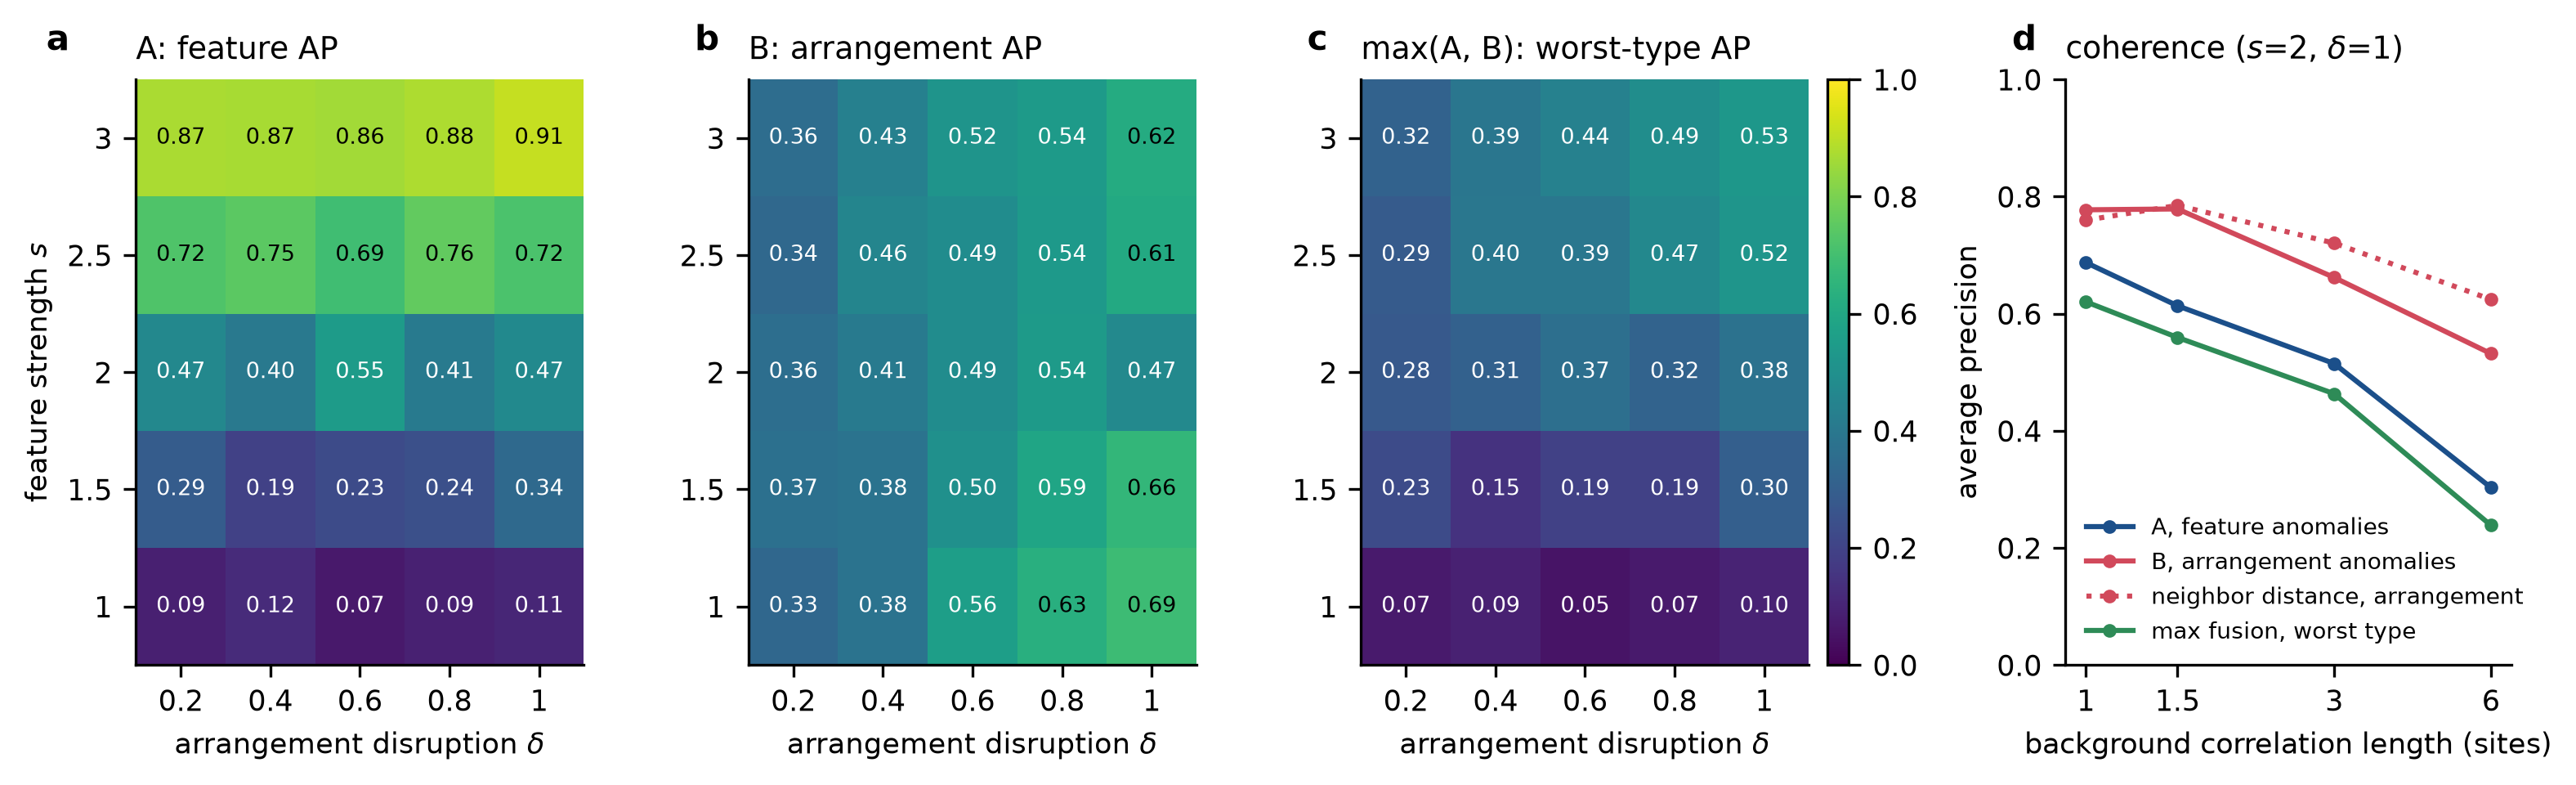
\includegraphics[width=\textwidth]{fig_phase.png}
\caption{Experiment A (G1, mixed lattices with $3\times3$ feature blocks, 20 lattices per cell). (a) Feature-anomaly AP of channel A, (b) arrangement-anomaly AP of channel B, (c) worst-type AP of max$(A,B)$ over feature strength $s$ and arrangement disruption $\delta$. (d) Dependence on the correlation length of the background at $s=2$, $\delta=1$.}
\label{fig:phase}
\end{figure*}

\subsection{Experiment B: fusion rules on the development generator}
Table~\ref{tab:dev} lists the mean per-type APs over the four mixed G1 conditions (30 lattices each). Single scores reached at most 0.21 in worst-type AP; the cohort-level selection, which picks one channel per cohort, did not improve on the channel it picked (0.06). Among the fusion rules, the site-wise maximum was best: max(rarity, $B$) 0.46, max$(A,B)$ 0.39, OR$(A,B)$ 0.30. Both adaptive rules were worse than the simple maximum (paired differences $-$0.18 [$-$0.22, $-$0.15] for lcOR and $-$0.41 [$-$0.44, $-$0.37] for relmax), so neither was adopted. Two comparisons were unfavorable to the channels proposed in the earlier version: on feature anomalies the unsmoothed rarity (0.59) and an isolation forest fitted per lattice (0.83) were above channel A (0.44), and on arrangement anomalies the Shekhar statistic (0.79) was above channel B (0.63). The generic pair max(isolation forest, Shekhar) reached 0.64, above the selected rule (0.46), but it was a comparator, not a candidate, under the declared protocol.

\begin{table}[t]
\caption{Experiment B (G1, four mixed conditions, 30 lattices each): mean AP for feature anomalies, arrangement anomalies and all anomalies, and the worst-type AP.}
\label{tab:dev}
\centering\footnotesize
\resizebox{\linewidth}{!}{\begin{tabular}{lcccc}
\toprule
Score or rule & Feature & Arrangement & All & Worst type\\
\midrule
Rarity (cohort, unsmoothed) & 0.59 & 0.05 & 0.26 & 0.05 \\
Channel A (similarity-weighted rarity) & 0.44 & 0.07 & 0.23 & 0.07 \\
Isolation forest & 0.83 & 0.05 & 0.34 & 0.05 \\
LOF & 0.19 & 0.05 & 0.13 & 0.05 \\
Channel B (directional disorder) & 0.06 & 0.63 & 0.50 & 0.06 \\
Shekhar statistic & 0.21 & 0.79 & 0.66 & 0.21 \\
Contextual LOF & 0.10 & 0.09 & 0.13 & 0.08 \\
OR(LOF, Shekhar) & 0.22 & 0.30 & 0.35 & 0.16 \\
\midrule
Cohort-level selection (tail index) & 0.06 & 0.63 & 0.50 & 0.06 \\
zmax of robust $z$ & 0.19 & 0.62 & 0.58 & 0.19 \\
lcOR (locally calibrated $B$) & 0.31 & 0.31 & 0.40 & 0.28 \\
relmax (reliability-weighted $B$) & 0.44 & 0.07 & 0.24 & 0.07 \\
OR$(A,B)$ & 0.31 & 0.35 & 0.43 & 0.30 \\
max$(A,B)$ & 0.39 & 0.47 & 0.53 & 0.39 \\
\midrule
max(rarity, $B$) [selected] & 0.53 & 0.48 & 0.58 & 0.46 \\
max(isolation forest, Shekhar) [comparator] & 0.82 & 0.64 & 0.77 & 0.64 \\
\bottomrule
\end{tabular}}
\end{table}

\subsection{Stage 1: the frozen rule failed on G2}
\label{sec:stage1}
Table~\ref{tab:stage1} gives the result on the 90 G2 lattices. The frozen max(rarity, $B$) reached a worst-type AP of 0.046, below the pre-declared generic comparators OR(LOF, Shekhar) (0.26), max(isolation forest, Shekhar) (0.22) and contextual LOF (0.16); the paired intervals of all three differences exclude zero. The failure has a clear cause: the cohort rarity was at chance on G2's feature anomalies (AP 0.04), whereas LOF fitted on each lattice found them (0.63). Every G2 lattice draws its own domain directions, so an embedding at $40^\circ$ from its local domain is unusual within its lattice but not in a cohort whose other lattices point in all directions. A rarity referenced to the cohort presupposes that the lattices share one normal distribution; G1 satisfied that assumption, G2 did not, and the development data could not reveal it.

\begin{table}[t]
\caption{Stage 1 (G2, three conditions pooled, 90 lattices): per-type AP, worst-type AP and the paired difference in worst-type AP of the frozen rule minus each comparator, with 95\% bootstrap interval.}
\label{tab:stage1}
\centering\footnotesize
\resizebox{\linewidth}{!}{\begin{tabular}{lcccc}
\toprule
Score or rule & Feature & Arrangement & Worst type & Frozen minus score\\
\midrule
Rarity (cohort) & 0.04 & 0.07 & 0.04 & -- \\
LOF & 0.63 & 0.07 & 0.07 & -- \\
Isolation forest & 0.27 & 0.07 & 0.07 & $-$0.02 [$-$0.03, $-$0.01] \\
Channel B & 0.06 & 0.35 & 0.06 & $-$0.02 [$-$0.02, $-$0.01] \\
Shekhar statistic & 0.06 & 0.40 & 0.06 & $-$0.02 [$-$0.03, $-$0.01] \\
Contextual LOF & 0.56 & 0.16 & 0.16 & $-$0.12 [$-$0.13, $-$0.10] \\
OR(LOF, Shekhar) & 0.48 & 0.26 & 0.26 & $-$0.21 [$-$0.24, $-$0.18] \\
Cohort-level selection & 0.06 & 0.31 & 0.06 & $-$0.01 [$-$0.02, 0.00] \\
max(isolation forest, Shekhar) & 0.22 & 0.30 & 0.22 & $-$0.18 [$-$0.22, $-$0.13] \\
max(rarity, $B$) [frozen] & 0.05 & 0.25 & 0.05 &  \\
\bottomrule
\end{tabular}}
\end{table}

\subsection{Stage 2: the revised rule on a new generator}
The post-hoc exploration (G1 and fresh G2 seeds) ranked max(isolation forest, Shekhar) first among the 24 pairs (mean worst-type AP 0.45; with channel B instead of the Shekhar statistic 0.38; with OR instead of max 0.27). That rule was frozen and tested on G3 (Table~\ref{tab:stage2}, Figs.~\ref{fig:maps} and~\ref{fig:confirm}). With shuffled regions it reached a worst-type AP of 0.53 (feature 0.96, arrangement 0.53), where every single score stayed at or below 0.09. Pooled over the two G3 conditions it was above every single score (paired differences between +0.25 and +0.29, all intervals above zero), above the stage-1 rule (+0.15 [+0.13, +0.16]), above OR(LOF, Shekhar) (+0.05 [+0.03, +0.07]) and level with contextual LOF ($-$0.01 [$-$0.04, +0.02]). On the fresh-seed replications it reached 0.65 on G1 and 0.19 on G2, where OR(LOF, Shekhar) was slightly better (0.21): the isolation forest finds G2's within-lattice anomalies less well than LOF.

Rotated patches were not detected by anything: the best arrangement AP of any score was 0.20, consistent with Proposition~\ref{prop:rot}, since only the patch borders differ from normal neighborhoods.

\begin{table*}[t]
\caption{Stage 2 (G3, 30 lattices per condition): per-type AP for shuffled regions and rotated patches, worst-type AP pooled over both conditions, and the paired difference in pooled worst-type AP of the frozen rule minus each score, with 95\% bootstrap interval.}
\label{tab:stage2}
\centering\footnotesize
\resizebox{\linewidth}{!}{\begin{tabular}{lcccccc}
\toprule
 & \multicolumn{2}{c}{Shuffled regions} & \multicolumn{2}{c}{Rotated patches} & Pooled & Frozen minus score\\
Score or rule & Feature & Arrangement & Feature & Arrangement & worst type & \\
\midrule
Cohort kNN rarity & 0.71 & 0.07 & 0.75 & 0.04 & 0.05 & +0.29 [+0.25, +0.34] \\
Within-lattice kNN rarity & 1.00 & 0.07 & 1.00 & 0.04 & 0.05 & +0.29 [+0.25, +0.34] \\
LOF & 1.00 & 0.07 & 1.00 & 0.04 & 0.05 & +0.29 [+0.24, +0.34] \\
Isolation forest & 1.00 & 0.07 & 1.00 & 0.04 & 0.05 & +0.29 [+0.25, +0.34] \\
Channel B & 0.06 & 0.47 & 0.06 & 0.05 & 0.06 & +0.29 [+0.23, +0.34] \\
Shekhar statistic & 0.09 & 0.67 & 0.11 & 0.19 & 0.10 & +0.25 [+0.19, +0.30] \\
Neighbor distance & 0.06 & 0.63 & 0.08 & 0.19 & 0.07 & +0.28 [+0.22, +0.33] \\
Contextual LOF & 0.97 & 0.52 & 0.95 & 0.20 & 0.36 & $-$0.01 [$-$0.04, +0.02] \\
OR(LOF, Shekhar) & 0.91 & 0.46 & 0.80 & 0.13 & 0.30 & +0.05 [+0.03, +0.07] \\
Cohort-level selection & 0.06 & 0.47 & 0.06 & 0.05 & 0.06 & +0.29 [+0.23, +0.34] \\
max(rarity, $B$) [stage-1 rule] & 0.63 & 0.36 & 0.54 & 0.04 & 0.20 & +0.15 [+0.13, +0.16] \\
max(isolation forest, Shekhar) [frozen] & 0.96 & 0.53 & 0.71 & 0.16 & 0.35 &  \\
\bottomrule
\end{tabular}}
\end{table*}

\begin{figure}[t]
\centering
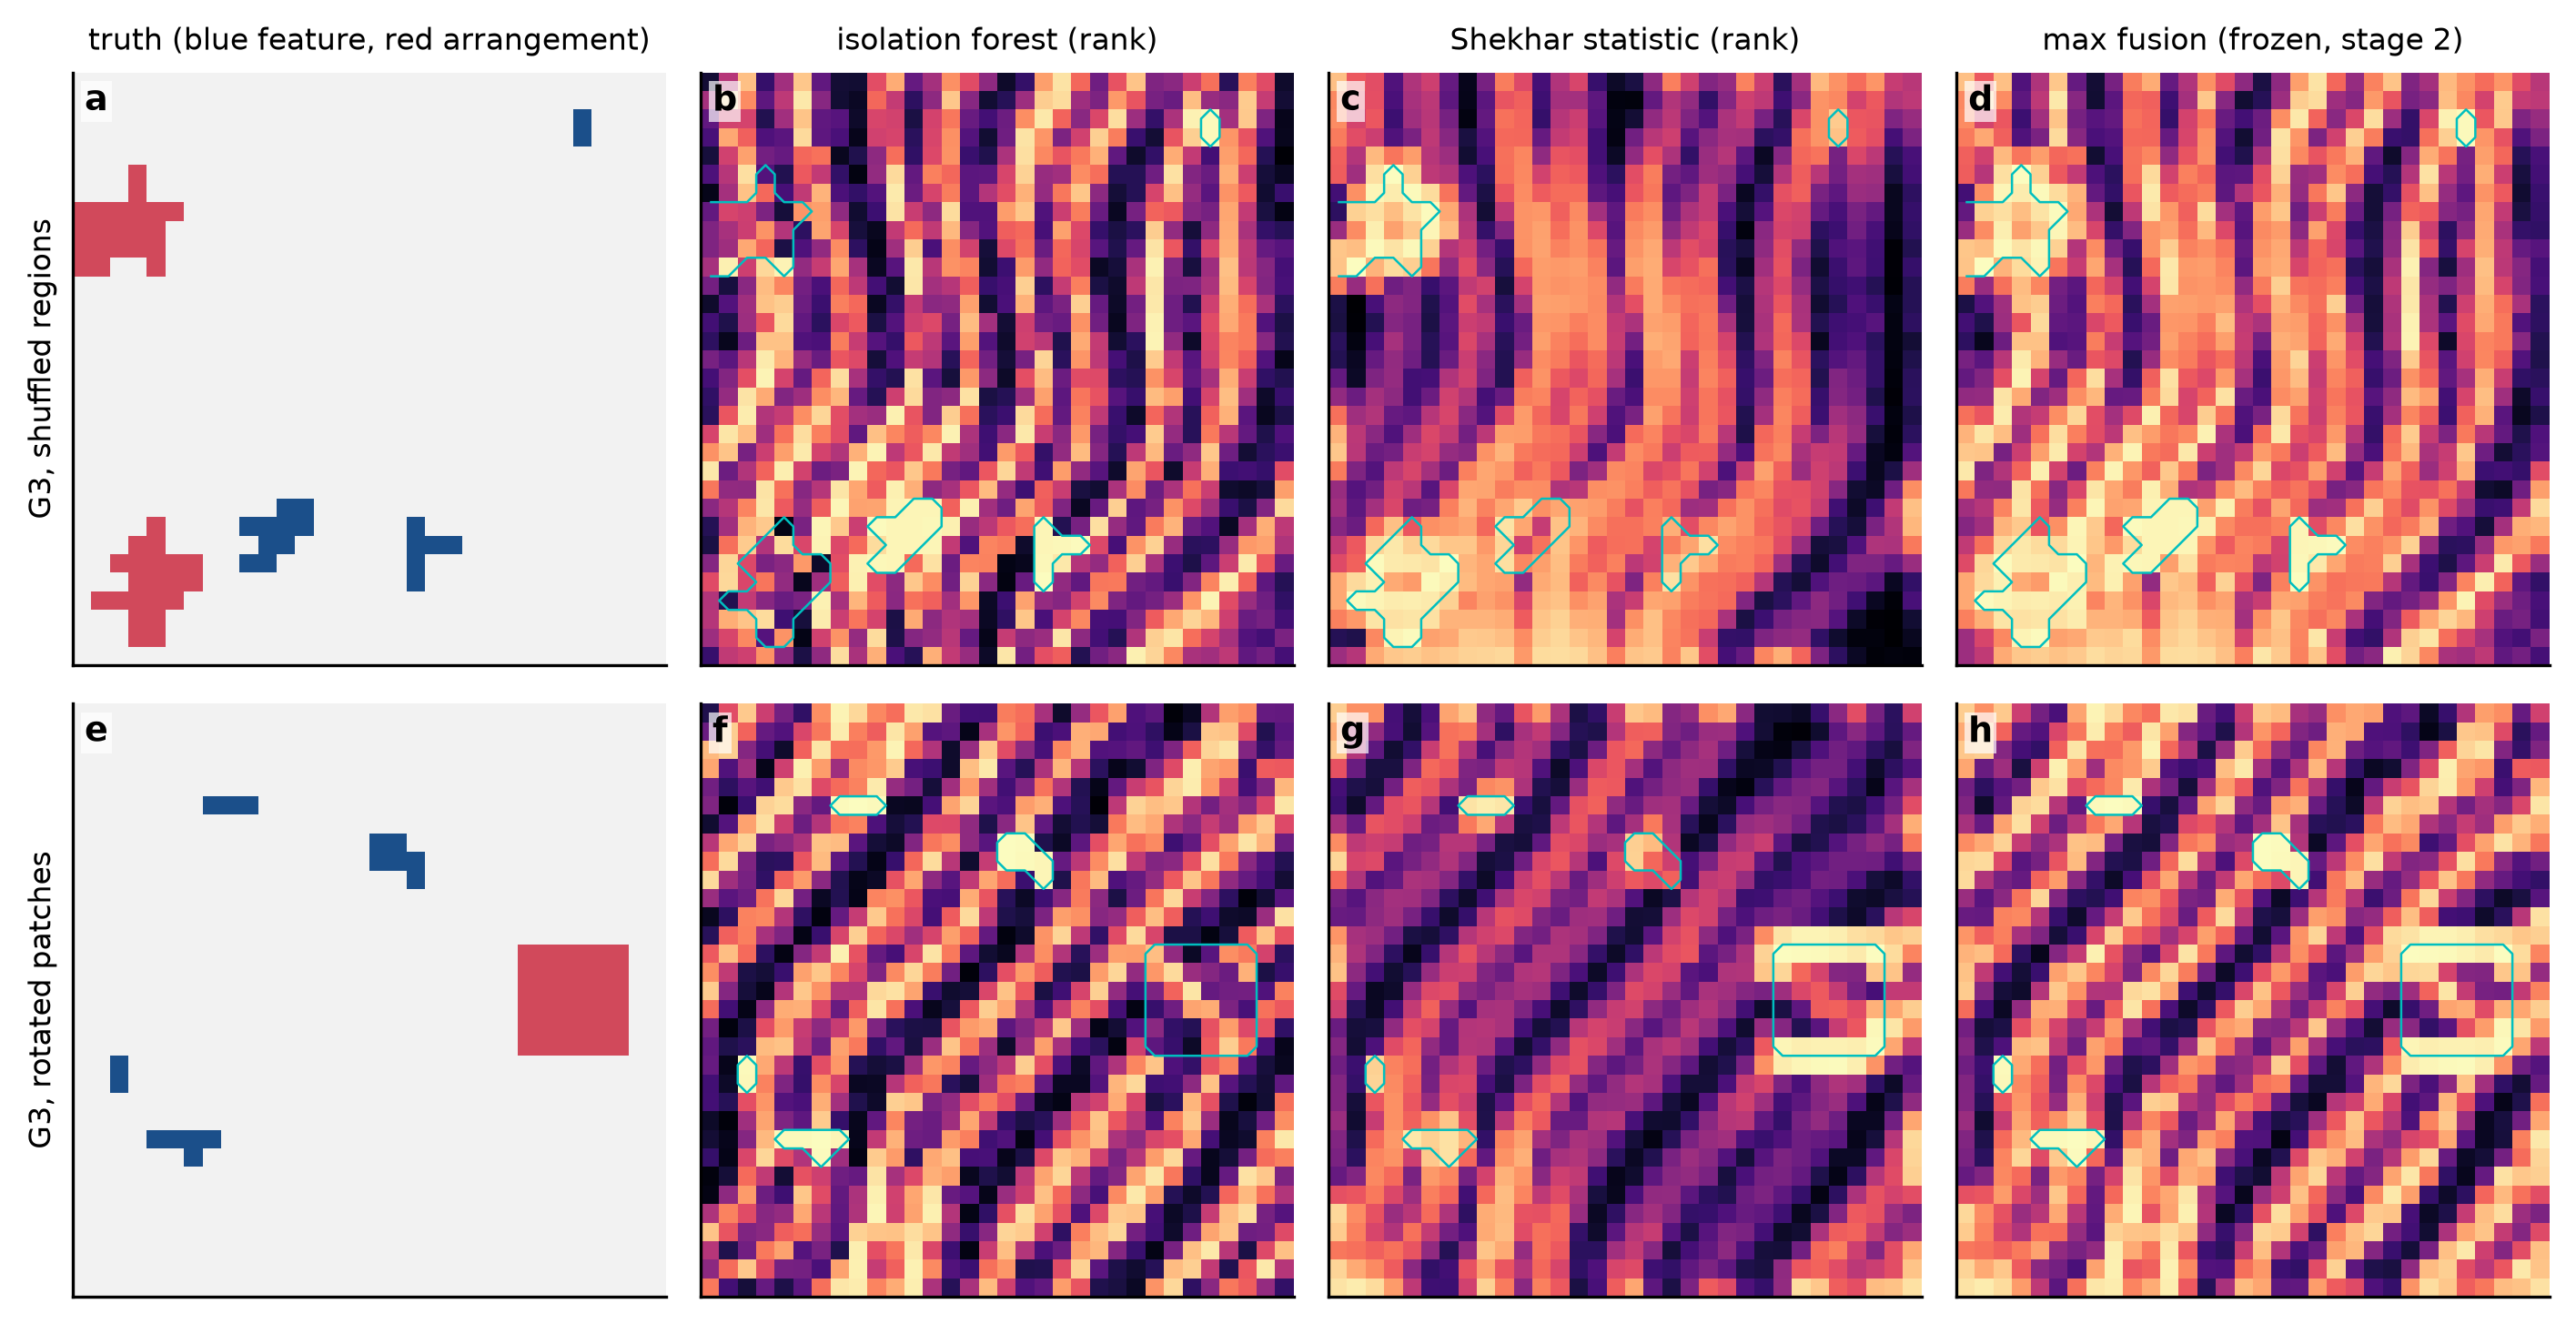
\includegraphics[width=\columnwidth]{fig_maps.png}
\caption{One G3 lattice with shuffled regions (top) and one with rotated patches (bottom): ground truth, cohort ranks of the isolation forest and of the Shekhar statistic, and the frozen stage-2 fusion; cyan contours mark the anomalies.}
\label{fig:maps}
\end{figure}

\begin{figure*}[t]
\centering
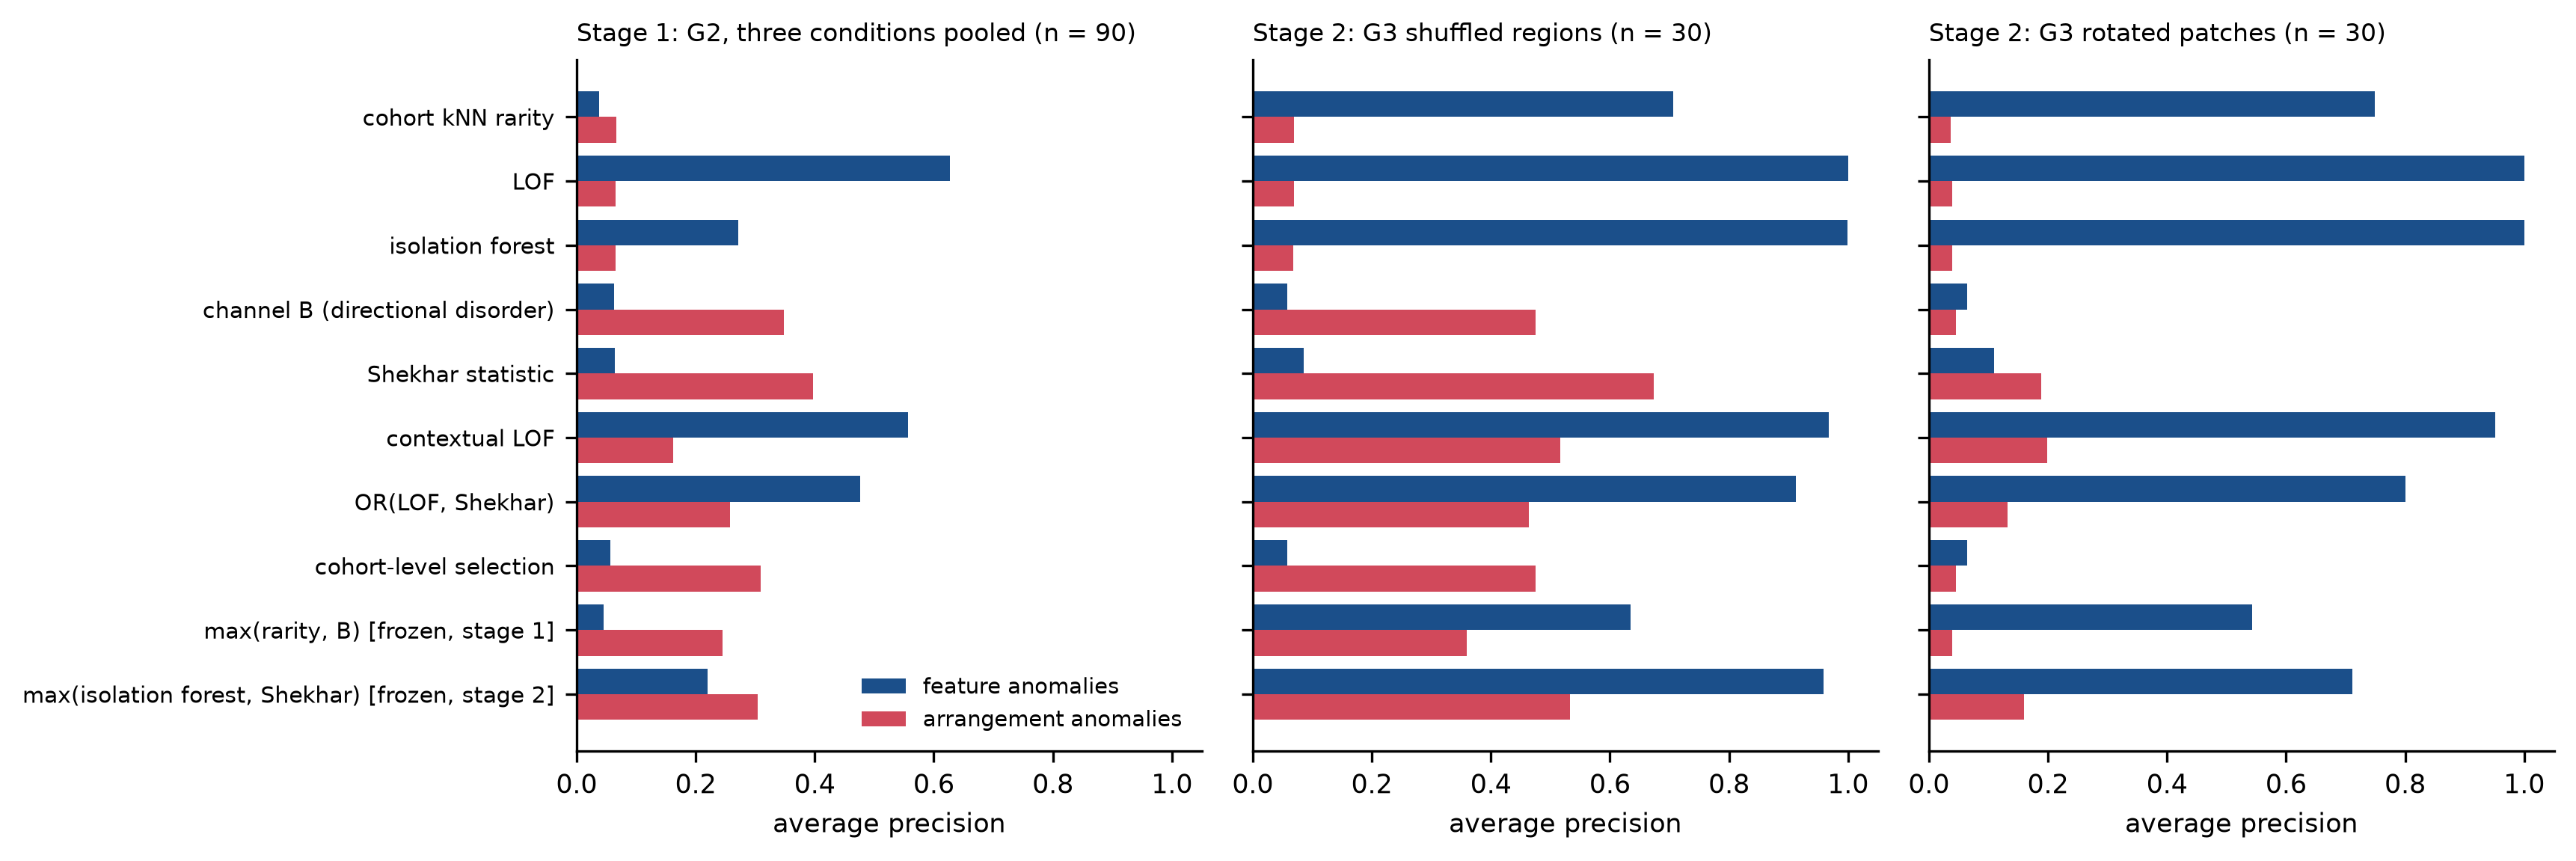
\includegraphics[width=\textwidth]{fig_confirm.png}
\caption{Per-type AP in the two confirmatory stages. Left: G2 (stage 1, 90 lattices); the stage-2 rule is shown for reference only, since it was chosen after this test. Middle and right: G3 (stage 2, 30 lattices each).}
\label{fig:confirm}
\end{figure*}

\subsection{Experiment D: robustness and cost}
Table~\ref{tab:robust} varies one factor at a time. On G3 with $32\times32$ lattices and $d\ge16$, the frozen rule reached a worst-type AP of 0.55--0.63 and was the best or within 0.01 of the best of the four fused rules in 12 of 13 settings (dimension, feature prevalence, window and noise); contextual LOF was better at noise 0.16 (0.59 against 0.52). At $d=2$ every method failed, because two dimensions cannot hold the texture manifold and its anomalies apart. Larger G3 lattices lowered every method (worst-type AP of the frozen rule 0.56, 0.41 and 0.11 for 32, 64 and 128 sites per side). This is a property of G3 rather than of the methods: its stripe phase is computed from absolute coordinates with a slowly varying orientation, so the background varies faster far from the origin (mean Shekhar statistic of anomaly-free lattices 0.29, 0.38 and 0.54); a scaling study needs a generator without this defect. On G2, every fused rule weakened as the background became less coherent, and OR(LOF, Shekhar) was above the frozen rule at every coherence level, because LOF finds G2's within-lattice anomalies better than the isolation forest. Computing all scores of this study took 0.4 s per $32\times32$ lattice at $d=16$, 0.6 s at $d=384$ and 4.1 s at $128\times128$ on a desktop computer; the isolation forest and LOF dominate the cost, and the spatial statistics are linear in the number of sites.

\begin{table}[t]
\caption{Experiment D: worst-type AP of four fused rules under one-at-a-time variation (10 lattices per setting; G3 with shuffled regions unless stated) and the time to compute all scores of the study per lattice.}
\label{tab:robust}
\centering\footnotesize
\resizebox{\linewidth}{!}{\begin{tabular}{llccccc}
\toprule
Factor & Value & max(IF, Shekhar) & max(rarity, $B$) & OR(LOF, Shekhar) & Contextual LOF & s/lattice\\
\midrule
dimension & 2 & 0.02 & 0.03 & 0.02 & 0.07 & 0.37 \\
 & 16 & 0.55 & 0.40 & 0.52 & 0.55 & 0.35 \\
 & 64 & 0.62 & 0.48 & 0.54 & 0.54 & 0.56 \\
 & 384 & 0.63 & 0.44 & 0.59 & 0.60 & 0.65 \\
\addlinespace
lattice size & 32 & 0.56 & 0.39 & 0.46 & 0.55 & 0.34 \\
 & 64 & 0.41 & 0.21 & 0.36 & 0.27 & 0.91 \\
 & 128 & 0.11 & 0.05 & 0.02 & 0.05 & 4.15 \\
\addlinespace
feature prevalence & 0.01 & 0.54 & 0.41 & 0.42 & 0.55 & 0.34 \\
 & 0.03 & 0.60 & 0.35 & 0.55 & 0.46 & 0.34 \\
 & 0.05 & 0.64 & 0.37 & 0.57 & 0.47 & 0.35 \\
\addlinespace
window & 3 & 0.59 & 0.39 & 0.53 & 0.56 & 0.34 \\
 & 5 & 0.59 & 0.17 & 0.54 & 0.56 & 0.36 \\
 & 7 & 0.54 & 0.06 & 0.46 & 0.50 & 0.35 \\
\addlinespace
coherence ($\kappa$ scale, G2) & 0.25 & 0.05 & 0.03 & 0.07 & 0.12 & 0.37 \\
 & 0.5 & 0.10 & 0.04 & 0.17 & 0.15 & 0.34 \\
 & 1.0 & 0.13 & 0.04 & 0.25 & 0.14 & 0.37 \\
 & 2.0 & 0.27 & 0.07 & 0.32 & 0.15 & 0.32 \\
\addlinespace
noise (G3) & 0.04 & 0.57 & 0.45 & 0.55 & 0.49 & 0.34 \\
 & 0.08 & 0.59 & 0.46 & 0.52 & 0.55 & 0.35 \\
 & 0.16 & 0.52 & 0.34 & 0.45 & 0.59 & 0.36 \\
 & 0.32 & 0.56 & 0.36 & 0.47 & 0.57 & 0.35 \\
\bottomrule
\end{tabular}}
\end{table}



\section{Discussion}
\label{sec:discussion}
\subsection{What the study establishes}
Within the stated assumptions and on controlled synthetic lattices, four findings hold across generators. (i) Feature scores and spatial-order scores detect different anomalies, and each is near chance on the other kind; Proposition~\ref{prop:perm} gives the reason for one direction, and the dispersion statistics' blindness to coherent unusual regions the other. (ii) When both kinds occur in the same lattice, choosing one score per cohort cannot work, and a site-wise maximum of cohort ranks is a strong, simple fusion: it beat OR, $z$-score maxima and two locally adaptive rules on the development generator, and its frozen form beat every single score and three fused baselines on a generator it had never seen. (iii) Whether a fixed aggregation window erases an anomaly is a geometric question that Proposition~\ref{prop:surv} answers in the strong-anomaly regime. (iv) No local, rotation-invariant statistic can see the interior of a rotated patch (Proposition~\ref{prop:rot}); such anomalies require orientation-aware or non-local models of the kind developed for logical anomalies in images \citep{Bergmann2022,Batzner2024}.

\subsection{Failure modes and limits of complementarity}
\emph{The reference of a feature score.} The stage-1 failure shows that a rarity score is only as good as its reference set: referencing it to the cohort assumes that all lattices share one normal distribution. When normality is defined per lattice (per image, per specimen), a within-lattice score such as LOF or an isolation forest is needed, and when the lattices do share a normal distribution, as with a fixed encoder in G3, both kinds of reference work. Which situation applies is a property of the data that should be checked before a detector is chosen, for example by comparing within-lattice and cross-lattice nearest-neighbor distances.

\emph{The spatial score.} The directional statistic of the earlier version did what Proposition~\ref{prop:wall} says (fewer responses at walls), but it was less sensitive than the plain Shekhar statistic to the arrangement anomalies of all three generators, and the selection preferred the latter. Its wall property would matter where walls are frequent and anomalies rare; in the present generators sensitivity mattered more.

\emph{The cost of fusion.} Proposition~\ref{prop:fuse} and the measured rates show the price: the false positives of the two channels add up, so the per-type AP of the maximum is below that of the better channel for each type (Table~\ref{tab:dev}). The maximum is the right choice when both kinds of anomaly matter; when only one does, the matching single channel is better. A fused score also does not say which kind of anomaly it found; keeping the two rank maps, as in Fig.~\ref{fig:maps}, does.

\emph{Background coherence.} A shuffle among nearly identical vectors is nearly invisible, so arrangement anomalies become harder, not easier, in very smooth backgrounds (Fig.~\ref{fig:phase}d); detectability depends on the variation of the background at the scale of the anomaly.

\subsection{What is not established}
All data are synthetic and were generated by the author of the analysis; G2 and G3 were written before their tests and frozen, but they are not independent of the author's assumptions. Nothing here shows performance on natural images, medical slides or industrial data, and the generators contain neither texture statistics nor encoder artefacts of real embeddings. The stage-2 rule was selected after the stage-1 failure on data that included G2, and its G2 replication is therefore not confirmatory. The comparison is limited to classical detectors; deep models trained on normal data were not included. Statistical uncertainty is over lattices of one generator; conclusions that should hold across generators rest on three generators only. G3 has a defect that limits it to small lattices: its texture becomes irregular far from the origin, so its results for lattices larger than $32\times32$ are not informative about scaling. What would refute the main conclusions: a generator with mixed anomalies on which a single score or a cohort-level choice matches the site-wise maximum, or a real data set on which the maximum of a feature and a spatial score does not improve the worst-type detection.

\subsection{Relation to the earlier version}
The earlier version reported that a cohort-level choice between channel A and channel B raised a lower-tail AP across fifteen test scenarios, most of which had been used during development. The present study replaces that design. Its results do not support the earlier recommendation: cohort-level selection fails on mixed lattices, and the two channels proposed earlier were outperformed by generic scores (an isolation forest and the Shekhar statistic) in the role they were designed for. What survives is the decomposition into a feature channel and a spatial channel, the occupancy explanation of aggregation loss, and the wall property of the directional statistic.



\section{Conclusions}
Feature rarity and spatial order are complementary sources of evidence on lattices of embeddings, and five elementary propositions bound what each, spatial aggregation and their fusion can detect. In controlled experiments with both kinds of anomaly in the same lattice, a site-wise maximum of the calibrated ranks of a within-lattice feature score and a neighbor-difference score was the most reliable label-free combination, and it survived a pre-registered test on a generator it had never seen. A first pre-registered rule failed because its feature score was referenced to a cohort that did not share one normal distribution; that failure, and the undetected rotated patches, mark the limits of local, marginal-plus-spatial detection. Testing these conclusions on real embedding lattices is the next step.



\section*{CRediT authorship contribution statement}
\textbf{Leon Sandler:} Conceptualization, Methodology, Software, Validation, Formal analysis, Investigation, Visualization, Writing -- original draft, Writing -- review \& editing.

\section*{Declaration of competing interest}
The author declares that he has no known competing financial interests or personal relationships that could have appeared to influence the work reported in this paper.

\section*{Funding}
This research did not receive any specific grant from funding agencies in the public, commercial, or not-for-profit sectors.

\section*{Data availability}
All data are synthetic and are regenerated by the code from the recorded seeds. Code, frozen protocols, result files and the version-control history with the freeze commits are openly available at \url{https://github.com/sandlerleon/MyUncleVision} (MIT license; modules \texttt{kbs\_study}, \texttt{kbs\_stage2}, \texttt{kbs\_robust}, \texttt{kbs\_props2}) and archived on Zenodo (\url{https://doi.org/10.5281/zenodo.24066260}).

\section*{Declaration of generative AI and AI-assisted technologies in the writing process}
During the preparation of this work the author used Claude (Anthropic) to assist with writing and testing the analysis code to the author's specification, with the figures and with language editing. The author reviewed and edited the content and takes full responsibility for the content of the published article.

\begin{thebibliography}{99}
\bibitem{Aggarwal2015} C.C. Aggarwal, S. Sathe, Theoretical foundations and algorithms for outlier ensembles, ACM SIGKDD Explor. Newsl. 17 (2015) 24--47. \url{https://doi.org/10.1145/2830544.2830549}.
\bibitem{Aggarwal2017} C.C. Aggarwal, Outlier Analysis, 2nd ed., Springer, Cham, 2017. \url{https://doi.org/10.1007/978-3-319-47578-3}.
\bibitem{Banerjee2005} A. Banerjee, I.S. Dhillon, J. Ghosh, S. Sra, Clustering on the unit hypersphere using von Mises--Fisher distributions, J. Mach. Learn. Res. 6 (2005) 1345--1382.
\bibitem{Batzner2024} K. Batzner, L. Heckler, R. K{\"o}nig, EfficientAD: accurate visual anomaly detection at millisecond-level latencies, in: Proc. IEEE/CVF Winter Conf. Appl. Comput. Vis. (WACV), 2024, pp. 127--137. \url{https://doi.org/10.1109/WACV57701.2024.00020}.
\bibitem{Bergmann2022} P. Bergmann, K. Batzner, M. Fauser, D. Sattlegger, C. Steger, Beyond dents and scratches: logical constraints in unsupervised anomaly detection and localization, Int. J. Comput. Vis. 130 (2022) 947--969. \url{https://doi.org/10.1007/s11263-022-01578-9}.
\bibitem{Breunig2000} M.M. Breunig, H.-P. Kriegel, R.T. Ng, J. Sander, LOF: identifying density-based local outliers, in: Proc. ACM SIGMOD Int. Conf. Manag. Data, 2000, pp. 93--104. \url{https://doi.org/10.1145/342009.335388}.
\bibitem{Chandola2009} V. Chandola, A. Banerjee, V. Kumar, Anomaly detection: a survey, ACM Comput. Surv. 41 (2009) 15:1--15:58. \url{https://doi.org/10.1145/1541880.1541882}.
\bibitem{Davis2006} J. Davis, M. Goadrich, The relationship between precision-recall and ROC curves, in: Proc. 23rd Int. Conf. Mach. Learn. (ICML), 2006, pp. 233--240. \url{https://doi.org/10.1145/1143844.1143874}.
\bibitem{Defard2021} T. Defard, A. Setkov, A. Loesch, R. Audigier, PaDiM: a patch distribution modeling framework for anomaly detection and localization, in: Pattern Recognition. ICPR International Workshops and Challenges, Lecture Notes in Computer Science, vol. 12664, Springer, Cham, 2021, pp. 475--489. \url{https://doi.org/10.1007/978-3-030-68799-1_35}.
\bibitem{Kriegel2011} H.-P. Kriegel, P. Kr{\"o}ger, E. Schubert, A. Zimek, Interpreting and unifying outlier scores, in: Proc. 2011 SIAM Int. Conf. Data Mining, 2011, pp. 13--24. \url{https://doi.org/10.1137/1.9781611972818.2}.
\bibitem{Kuwahara1976} M. Kuwahara, K. Hachimura, S. Eiho, M. Kinoshita, Processing of RI-angiocardiographic images, in: K. Preston, M. Onoe (Eds.), Digital Processing of Biomedical Images, Plenum Press, New York, 1976, pp. 187--202. \url{https://doi.org/10.1007/978-1-4684-0769-3_13}.
\bibitem{Liu2008} F.T. Liu, K.M. Ting, Z.-H. Zhou, Isolation forest, in: Proc. 8th IEEE Int. Conf. Data Mining (ICDM), 2008, pp. 413--422. \url{https://doi.org/10.1109/ICDM.2008.17}.
\bibitem{Mardia2000} K.V. Mardia, P.E. Jupp, Directional Statistics, Wiley, Chichester, 2000.
\bibitem{Pang2021} G. Pang, C. Shen, L. Cao, A. van den Hengel, Deep learning for anomaly detection: a review, ACM Comput. Surv. 54 (2022) 38:1--38:38. \url{https://doi.org/10.1145/3439950}.
\bibitem{Roth2022} K. Roth, L. Pemula, J. Zepeda, B. Sch{\"o}lkopf, T. Brox, P. Gehler, Towards total recall in industrial anomaly detection, in: Proc. IEEE/CVF Conf. Comput. Vis. Pattern Recognit. (CVPR), 2022, pp. 14298--14308. \url{https://doi.org/10.1109/CVPR52688.2022.01392}.
\bibitem{Rousseeuw1993} P.J. Rousseeuw, C. Croux, Alternatives to the median absolute deviation, J. Am. Stat. Assoc. 88 (1993) 1273--1283. \url{https://doi.org/10.1080/01621459.1993.10476408}.
\bibitem{Ruff2021} L. Ruff, J.R. Kauffmann, R.A. Vandermeulen, G. Montavon, W. Samek, M. Kloft, T.G. Dietterich, K.-R. M{\"u}ller, A unifying review of deep and shallow anomaly detection, Proc. IEEE 109 (2021) 756--795. \url{https://doi.org/10.1109/JPROC.2021.3052449}.
\bibitem{Schubert2014} E. Schubert, A. Zimek, H.-P. Kriegel, Local outlier detection reconsidered: a generalized view on locality with applications to spatial, video, and network outlier detection, Data Min. Knowl. Discov. 28 (2014) 190--237. \url{https://doi.org/10.1007/s10618-012-0300-z}.
\bibitem{Shekhar2003} S. Shekhar, C.-T. Lu, P. Zhang, A unified approach to detecting spatial outliers, GeoInformatica 7 (2003) 139--166. \url{https://doi.org/10.1023/A:1023455925009}.
\bibitem{Song2007} X. Song, M. Wu, C. Jermaine, S. Ranka, Conditional anomaly detection, IEEE Trans. Knowl. Data Eng. 19 (2007) 631--645. \url{https://doi.org/10.1109/TKDE.2007.1009}.
\bibitem{Tomasi1998} C. Tomasi, R. Manduchi, Bilateral filtering for gray and color images, in: Proc. 6th Int. Conf. Comput. Vis. (ICCV), 1998, pp. 839--846. \url{https://doi.org/10.1109/ICCV.1998.710815}.
\end{thebibliography}


\end{document}
